%!TEX root = ../main.tex
\chapter{Hypothesentests}
\section{Binomialtest}
Man beginnt mit einer Hypothese, zum Beispiel möchte man Prüfen ob die Trefferwahrscheinlichkeit einer Binomialverteilung tatsächlich einem bestimmten Wert $p_0$ entspricht.
Die Nullhypothese wäre dann $H_0: p=p_0$, das heißt keine Besonderheiten. Wir führen später eine Stichprobe durch und entscheiden uns dann abhängig von dessen Ergebnis für oder gegen $H_0$.

Nun kann man sich entscheiden wie man die Gegenhypothese aufstellen will. Abhängig davon ergibt sich die Testcharakteristik
\begin{enumerate}
	\item Linksseitiger Test: $H_1: p<p_0$
	\item Rechtsseitiger Test: $H_1: p>p_0$
	\item Beidseitiger Test: $H_1: p\neq p_0$
\end{enumerate}
Um $p\in\Theta=(0,1)$ einer $\binomial(n,p)$-Verteilung zu testen sehen die wichtigen Werte in etwa so aus (kann insbesondere bei $\Theta$ abweichen)
\begin{center}
	\begin{tabular}{r|ccc}
		&linksseitig&gemeinsam&rechtsseitig\\\hline
		Annahmebereich:&$\Theta_0=[p_0,1)$&$\Big|$&$\Theta_0=(0,p_0]$\\
		Ablehnungsbereich:&&$\Theta_1=(0,1)\setminus\Theta_0$&\\
		Kritischer Punkt:&\makecell{$k^\ast$ maximal mit\\ $P_{p_0}(X\leq k^\ast)\leq\alpha$}&$\Bigg|$&\makecell{$k^\ast$ minimal mit\\ $P_{p_0}(X\geq k^\ast)\leq\alpha$}\\
		Kritischer Bereich:&$\mathcal K_1=\simpleset{0,\ldots,k^\ast}$&$\Big|$&$\mathcal K_1=\simpleset{k^\ast,\ldots,n}$\\
		Gütefunktion:&&$g(p)=P_p(X\in\mathcal K_1)$&\\
	\end{tabular}
\end{center}
Im Beispiel von oben wäre $\Theta_0=\simpleset{p_0}$ und $\Theta_1$ abhängig von der Testcharakteristik so zum Beispiel für einen rechtsseitigen Test $\Theta_1=(p_0,1)$.

Den Ablehnungsbereich bestimmt man mithilfe der Gütefunktion an der Stelle $p_0$. Das heißt man bestimmt $k^\ast$ als Grenze des $\mathcal K_1$ so, dass
\begin{equation*}
	\forall p\in\Theta_0 : g(p)=P_{p}(X\in\mathcal K_1)\overset!\leq\alpha.
\end{equation*}
Das heißt insbesondere, dass die Wahrscheinlichkeit eine falsche Aussage für $H_1$ zu treffen kleiner als $\alpha$ ist (Fehler 1. Art). Für einen rechtsseitigen Test könnte eine Gütefunktion wie folgt aussehen
\begin{center}
	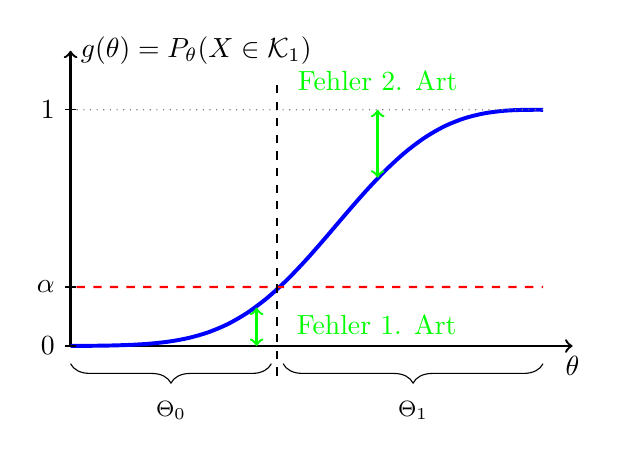
\begin{tikzpicture}[scale=0.75]
		\draw[->, line width=0.3mm] (0,0) to (8.5,0) node[below] {$\theta$};
		\draw[->, line width=0.3mm] (0,0) to (0,5) node[right] {$g(\theta)=P_\theta(X\in \mathcal K_1)$};		

		\draw[line width=0.5mm,scale=1,domain=0:8,smooth,variable=\x,blue] plot ({\x},{4*exp((\x/4-2)^3)});
		%\draw[line width=0.5mm,scale=1,domain=4:8,smooth,variable=\x,blue] plot ({\x},{-3.12*exp(-(\x-4))+4});
		
		\draw (0,0) node (null) [rectangle,inner sep = 0pt,minimum size = 0pt,minimum width=4pt,draw, label={left:$0$}] {};
		\draw (0,4) node (eins) [rectangle,inner sep = 0pt,minimum size = 0pt,minimum width=4pt,draw, label={left:$1$}] {};
		\draw (0,1) node (alpha) [rectangle,inner sep = 0pt,minimum size = 0pt,minimum width=4pt,draw, label={left:$\alpha$}] {};

		\draw[red, dashed, line width=0.3mm] (alpha) -- (8,1);
		\draw[gray, dotted] (eins) -- (8,4);

		\draw[black, line width=0.3mm, dashed] (3.5,-0.5) -- (3.5,4.5);
			
		\draw [decorate,decoration={brace,amplitude=7pt}]
		(3.4,-0.3) -- (0,-0.3) node [black,midway, yshift=-17pt] 
		{\footnotesize $\Theta_0$};

		\draw [decorate,decoration={brace,amplitude=7pt}]
		(8,-0.3) -- (3.6,-0.3) node [black,midway, yshift=-17pt] 
		{\footnotesize $\Theta_1$};

		%Fehler 1. Art
		\draw [arrows=<->, green, line width=0.3mm] (3.15,0) -- (3.15,0.65);
		\draw (3.5,0.35) node (null) [label={right:{\color{green}Fehler 1. Art}}] {};
		

		%Fehler 2. Art
		\draw [arrows=<->, green, line width=0.3mm] (5.2,2.85) -- (5.2,4);
		\draw (5.2,4) node (null) [label={above:{\color{green}Fehler 2. Art}}] {};
	\end{tikzpicture}	
\end{center}
Abhängig von der durchgeführten Stichprobe entscheidet man sich für die wahrscheinlichere Hypothese. Das heißt falls $X(\omega)\in\mathcal K_1$ gilt, steht die Stichprobe im widerspruch zu $H_0$ und der Parameter $p_0$ ist sehr unwahrscheinlich, so wird $H_0$ zugunsten von $H_1$ verworfen.

Ist allerdings $X(\omega)\in\mathcal K_0$, so kann die Nullhypothese nicht verworfen werden.
\paragraph{Fehlerarten}
\begin{center}
	\begin{tabular}{r|cc}
		&\multicolumn{2}{c}{Realität}\\
		&$H_0$ gilt&$H_1$ gilt\\\hline
		$H_0$ nicht verworfen&Spezifität&\makecell{Fehler 2. Art\\ false negative}\\
		$H_0$ verworfen&\makecell{Fehler 1. Art\\ false positive}&Sensitivität
	\end{tabular}
\end{center}
Der Fehler erster Art beschreibt die Wahrscheinlichkeit, die Nullhypothese fälschlicherweise abzulehnen
\begin{equation*}
	P_{p_0}(X\in \mathcal K_1),
\end{equation*}
er ist beschränkt durch $\alpha$. Verwirft man also $H_0$, so stimmt diese Aussage mit Wahrscheinlichkeit $(1-\alpha)$.


\subsection{Approximativer Binomialtest}
Der approximative Binomialtest unterschiedet sich nur in der Bestimmung von $k^\ast$. Dies geschieht hier durch den zentralen Grenzwertsatz, man führt die Binomialverteilung auf eine Standardnormalverteilung zurück und verfährt analog zum Gaußtest. Es gilt für $X\sim\binomial(n,p)$
\begin{equation*}
	\frac{X-np}{\sqrt{np(1-p)}}\sim\norm(0,1)
\end{equation*}
Man bestimmt $k^\ast$ wie folgt
\begin{align*}
	\text{linksseitiger Test}&&&&\text{rechtsseitiger Test}\\
	P_{p_0}(X\leq k^\ast)&\leq \alpha &&& P_{p_0}(X\geq k^\ast)&\leq \alpha\\
	\Phi\left(\frac{k^\ast-np_0}{\sqrt{np_0(1-p_0)}}\right)&\leq \alpha &&&\Phi\left(\frac{k^\ast-np_0}{\sqrt{np_0(1-p_0)}}\right)&\leq 1-\alpha\\
	\frac{k^\ast-np_0}{\sqrt{np_0(1-p_0)}}&\leq z_{\alpha} &&&\frac{k^\ast-np_0}{\sqrt{np_0(1-p_0)}}&\leq z_{1-\alpha}
\end{align*}
Dann wird wie bei einem normalen Binomialtest entschieden.

\section{Gaußtest (Test mit der Normalverteilung)}
Wir wollen mit dem Mittelwert der Normalverteilung einen Hypothesentest durchführen. Das heißt also zum Beispiel prüfen ob der Mittelwert tatsächlich einem erwarteten Wert $\mu$ entspricht.
\begin{enumerate}
	\item Wir verwenden hierfür die Teststatistik $\overline X=\frac1n\sum_{i=1}^n X_i$ als Schätzer für den Mittelwert. Wir benötigen außerdem den Standardfehler $\sigma_{\overline X}=\sqrt{\frac{\sigma^2}{n}}$ um auf die Standardnormalverteilung reduzieren zu können.
	\item Nun führen den Test auf eine Standardnormalverteilung zurück, indem wir die folgende Zufallsvariable festlegen
	\begin{equation*}
		Z=\frac{\overline X-\mu}{\frac{\sigma}{\sqrt n}}\sim\norm(0,1).
	\end{equation*}
	\item Wir können nun die Quantile $z_p$ der Standardnormalverteilung aus einer Tabelle ablesen.
	Dann wird der Ablehnungsbereich $\Theta_1$ entsprechend dem Signifikanzniveau $\alpha$ wie folgt bestimmt
	\begin{center}
		\begin{tabular}{c|c|c}
			linksseitiger Test&rechtsseitiger Test&beidseitiger Test\\\hline
			$\Theta_1=(-\infty, z_{\alpha}]$&$\Theta_1=[z_{1-\alpha},\infty)$&$\Theta_1=(-\infty, z_{\alpha/2}]+[z_{1-\alpha/2},\infty)$
		\end{tabular}
	\end{center}
	\item Als letztes muss man noch prüfen, ob der beobachtete Wert aus der Teststatistik im Ablehnungsbereich liegt. Das heißt, falls
	\begin{equation*}
	 	\frac{\overline X-\mu}{\frac{\sigma}{\sqrt n}}\in \Theta_1
	\end{equation*}
	für die gegebene Stichprobe gilt, so wird $H_0$ zum gegebenen Signifikanzniveau verworfen.
\end{enumerate}

\section{Chi-Quadrat-Anpassungstest}
Der $\chi^2$-Anpassungstest testet eine gegebene Stichprobe auf die zugrundeliegende Verteilung. Die Fragestellung ist also \glqq Sind die gegebenen Werte $\ast$-verteilt?\grqq

Stehen $n$ unabhängige, identische Wiederholungen $X_i$ des Merkmals $X=\simpleset{1,2,\ldots,k}$ zur Verfügung, kann die folgende Tabelle (gedanklich) aufgestellt werden
\begin{center}
	\begin{tabular}{r|cccc|l}
		Ausprägung&$1$&$2$&$\cdots$&$k$&\\\hline
		absolute Häufigkeit&$h_1$&$h_2$&$\cdots$&$h_k$&$\sum=n$\\
		erwartete W.-keit&$\pi_1$&$\pi_2$&$\cdots$&$\pi_k$&$\sum=1$
	\end{tabular}
\end{center}
Dabei ist dann die Nullhypothese 
\begin{equation*}
	H_0\text{ die Elemente sind verteilt wie $X$, d.h.} \forall i\enspace P(X=i)=\pi_i.
\end{equation*}
Man erhält also durch $\tilde h_i =n*\pi_i$ die erwartete Häufigkeit, wenn die Verteilung von $X$ zugrunde liegt.
Wir testen nun simultan alle Abweichungen der $h_i$ von den erwarteten $\tilde h_i$ mit der $\chi^2$-Teststatistik
\begin{equation*}
	\chi^2=\sum_{i=1}^k\frac{(h_i-n*\pi_i)^2}{n*\pi_i}=\sum_{i=1}^k\frac{(h_i-n*\tilde h_i)^2}{\tilde h_i}.
\end{equation*}
Ist dieser Wert groß, so handelt es sich höchstwahrscheinlich nicht um die richtige Verteilung.

Da die Zufallsvariable (Teststatistik) $\chi^2$ nun auch $\chi^2(k-1)$-verteilt ist, können wir mit dem $(1-\alpha)$-Quantil der $\chi^2(k-1)$-Verteilung den Ablehnungsbereich bestimmen, dabei ist $\alpha$ das Signifikanzniveau.
Das heißt, wir verwerfen $H_0$ falls
\begin{equation*}
	\chi^2>\chi^2_{(1-\alpha)}(k-1)
\end{equation*}
gilt. Dann kann man mit Sicherheit $1-\alpha$ sagen, die Urliste ist nicht verteilt wie $X$.

\section{Chi-Quadrat-Unabhängigkeitstest}
Der $\chi^2$-Unabhängigkeitstest testet eine Stichprobe von zwei Zufallsvariablen $(X,Y)$ auf Unabhängigkeit.
Die Nullhypothese lautet also
\begin{equation*}
	H_0:\ X\text{ und }Y\text{ sind unabhängig, d.h. }\forall i,j\enspace P(X=i, Y=j)=P(X=i)*P(Y=j).
\end{equation*}
Aus der Stichprobe erhält man wieder eine Tabelle der absoluten Häufigkeiten mit den Randhäufigkeiten
\begin{center}
	\begin{tabular}{c|cccc|c}
		&$Y=1$&$Y=2$&$\cdots$&$Y=m$&\\\hline
		$X=1$&$h_{11}$&$h_{12}$&&$h_{1m}$&$h_{1*}$\\
		$X=2$&$h_{21}$&$h_{22}$&&$h_{2m}$&$h_{2*}$\\
		$\vdots$&&&$\ddots$&\\
		$X=k$&$h_{k1}$&$h_{k2}$&&$h_{km}$&$h_{k*}$\\\hline
		&$h_{*1}$&$h_{*2}$&&$h_{*m}$&$n$
	\end{tabular}
\end{center}
Aus den Randhäufigkeiten bestimmt man dann die erwarteten Häufigkeiten der Merkmalsausprägungen bei unabhängigen Merkmalen
\begin{equation*}
	\tilde h_{ij}=\frac{h_{i*}*h_{*j}}{n}
\end{equation*}
Damit bestimmt man schließlich wieder die Chi-Quadrat-Teststatistik
\begin{equation*}
	\chi^2=\sum_{i=1}^k \sum_{j=1}^m \frac{(h_{ij}-\tilde h_{ij})^2}{\tilde h_{ij}}.
\end{equation*}
Den so erhaltenen Wert vergleicht man wiederum mit dem $1-\alpha$-Quantil. Falls
\begin{equation*}
	\chi^2 > \chi^2_{(1-\alpha)}((k-1)*(m-1))
\end{equation*}
gilt, so ist die Nullhypothese zu verwerfen.